\documentclass[a4paper]{article}
\usepackage[utf8]{inputenc}
\usepackage[russianb]{babel}
\usepackage{amsthm}
\usepackage{amsfonts,amssymb}
\usepackage{graphicx}
\usepackage{amsmath}
\usepackage{enumitem}
\Russian

\setlength{\hoffset}{-15mm}
\setlength{\voffset}{-15mm}
\setlength{\textheight}{235mm}
\setlength{\textwidth}{150mm}
\setlength{\oddsidemargin}{20mm}
\setlength{\oddsidemargin}{20mm}

\linespread{1.25}
\frenchspacing
\setlist[enumerate,1]{leftmargin=5mm}

\newcommand{\Qp}{\mathbb{Q}_p}
\newcommand{\Zp}{\mathbb{Z}_p}
\newcommand{\Fp}{\mathbb{F}_p}
\newcommand{\Fq}{\mathbb{F}_q}
\newcommand{\Z}{\mathbb{Z}}
\newcommand{\ML}{\mathfrak{M}_L}
\newcommand{\MLO}{\mathfrak{M}_{L_1}}
\newcommand{\MF}{\mathfrak{M}_F}
\newcommand{\MK}{\mathfrak{M}_K}
\newcommand{\Mk}{\mathfrak{M}_k}
\newcommand{\Ok}{\mathfrak{O}_k}
\newcommand{\OK}{\mathfrak{O}_K}
\newcommand{\OF}{\mathfrak{O}_F}
\newcommand{\ON}{\mathfrak{O}_N}
\newcommand{\OTK}{\mathfrak{O}_{T_K}}
\newcommand{\OL}{\mathfrak{O}_L}
\newcommand{\OLO}{\mathfrak{O}_{L_1}}
\newcommand{\OTL}{\mathfrak{O}_{T_L}}
\newcommand{\RL}{\mathfrak{R}_L}
\newcommand{\val}{\mathfrak{v}}
\newcommand{\olval}{\overline{\mathfrak{v}}}
\newcommand{\pK}{\mathfrak{p}_K}
\newcommand{\Rb}{\mathbb{R}}
\newcommand{\Leq}{\leqslant}
\newcommand{\Geq}{\geqslant}
\newcommand{\Zero}{\mathbb{0}}

\newtheorem{note}{Замечание}
\newtheorem{proposition}{Предложение}
\newtheorem{lemma}{Лемма}
\newtheorem{oldtheorem}{Теорема}
\newtheorem{theorem}{Теорема}


\title{Testo}
\author{Sergey Vlassiev}
\date{\today}
\begin{document}
\section{Используемые обозначения}
\paragraph{}
Мы будем использовать следующие обозначения.\\
$q=p^f$, где $p\neq2$ --- простое число.\\
$K$ --- многомерное локальное поле такое, что существует цепочка полей 
$$K=k^{(n)}, k^{(n-1)},\dots,k^{(1)},k^{(0)}=\Fq,$$
где $k^{(i)}$ при $1\Leq i\Leq n$ является полным дискретно нормированным полем с полем вычетов $k^{(i-1)}$.\\
Набор $t_n,\dots,t_1$ --- система локальных параметров поля $K$, то есть $t_i$ является единицей в полях $K,k^{(n-1)},\dots,k^{(i+1)}$ и при этом в поле $k^{(i)}$ является простым элементом. Таким образом, $t_n=\pi$ --- простой элемент локального поля $K$.\\
$\overline{\val_K}=\olval=(\val_1,\dots,\val_n):K^*\rightarrow\Z^n$ --- нормирование ранга $n$ в $K$. Здесь $\val_n(a)=\val_{k^{(n)}}(a)$, а для $1\Leq i<n$
$$v_i(a) = \val_{k^{(i)}} \left( \overline {a \over { t_n^{\val_n(a)} \ldots t_{i+1}^{\val_{i+1}(a)} } } \right),$$\\
$$v_n(a)=\val_{k^{(n)}}(a).$$\\
$\OK=\{a\in K^*\ |\ \overline{\val}(a)\Geq0\}$ --- кольцо нормирования, которое не зависит от выбора системы локальных параметров.\\
$\MK=\mathfrak{M}=\{a\in\OK\ |\ \overline{\val}(a)>0\}$ --- максимальный идеал кольца нормирования.\\
$e_K$ --- индекс ветвления поля $K$ относительно нормирования $\val=\val_n$, то есть $\val(p)=e_K$.\\
$\overline{e_K}$ --- индекс ветвления поля $K$ относительно нормирования $\olval$.\\
Введём обозначение: $\pK(r_l,\dots,r_n)=\{a\in K\ |\ (v_l(a),\dots,v_n(a))\Geq(r_l,\dots,r_n)\}$. Мы считаем, что группа $\Z^n$ лексикографически упорядоченна: $(i_1,\dots,i_n)<(j_1,\dots,j_n)$, если для наибольшего индекса $l$, для которого $i_l\neq j_l$, выполняется $i_l<j_l$. Если $(r_l,\dots,r_n)>(0,\dots,0)$, то $\pK(r_l,\dots,r_n)$ --- идеал в $\OK$. Более того, любой идеал в $\OK$ может быть представлен в виде $\pK(r_l,\dots,r)n)$.\\
Рассмотрим теперь набор мультииндексов $I\subset\Z^n$, будем называть набор $I$ допустимым, если для любых $i_n,\dots,i_{l+1}\ 1\Leq l\Leq n$ найдётся целое число $i$ такое, что из того, что $\overline{r}=(r_1,\dots,r_l,i_{l+1},\dots,i_n)\in I$ следует $r_l\Geq i$. Согласно работе $\cite{K_Teorii}$, если мы зафиксируем $B$ ---произвольную систему представителей $\Fq$ в $K$, то
$$\forall s \in K\ s= \sum_{\overline{r} \in I} \alpha_{\overline{r}} t_n^{r_n} \ldots t_1^{r_1},$$
где $I$ --- допустимый набор, а $\alpha_{\overline{r}}\in B$.\\

\pagebreak

Рассмотрим многомерное локальное поле $K=k^{(n)}, k^{(n-1)},\dots,k^{(1)},k^{(0)}=\Fq,$ в случае, когда $k^{(1)} = k$ --- одномерное локальное поле характеристики ноль (конечное расширение $\Qp$). В этом случае $K = k((t_2))\dots((t_n)).$ 

Пусть $L$ --- конечное расширение поля $K$ без высшего ветвления, тогда $L = L^{(1)}((T_2))\dots((T_n)),$ где $L_1$ --- конечное расширение поля $k$. При этом $(\pi = t_1, t_2, \dots, t_n)$ и $(\Pi = T_1, T_2, \dots, T_n)$ --- суть системы локальных параметров в полях $K$ и $L$ соответственно. И Пусть $\RL$ --- набор представителей Тейхмюллера в поле $L$.\\

Одномерная формальная группа $F(X,Y)\in\OK[[X,Y]]$ высоты $h$ определяет фильтрацию Лютц на модуле $F(\ML)$.

В одномерном случае в предложении 4 мы получили образующие модуля $F(\ML)$. В случае многомерных полей $L/K$ этот результат получается аналогичным образом. Действительно, результаты работы \cite{book2} могут быть применены и к многомерным локальным полям $L/K$ при условии малости абсолютного индекса ветвления поля $K$: $e_0=e(K/\Qp)<p$. Тогда очевидно, что рассуждения об образующих модуля $F(\ML)$ могут быть повторены для многомерного случая. Таким образом, мы получим, что, если поле $L$ не содержит нетривиальных корней изогении $[p]_F$, а $e_0 < p$, то любой элемент $\alpha\in(\ML)$ единственным образом записывается в виде суммы $\alpha={\sum}_{(F)}^*[p]_F^r\varepsilon_s(\theta_{s,r})$. Откуда, с учётом предложения 2, следует предложение 4 для многомерного случая.

С помощью предложения 5, взятого из работы \cite{GroupsClassification} мы получили обобщённую функцию Артина-Хассе. В работе \cite{GroupsClassification} рассматриваются обобщённые локальные поля, то есть этот результат применим и для случая многомерных локальных полей $L/K$. При этом поле $k^{(1)}=k$ не обязательно должно быть конечным расширением $\Qp$, рассуждения верны для полных дискретно нормированных полей с совершенным полем вычетов полей. Тогда для многоменрного случая будет верно и предложение 6 о свойствах обобщённой функции Артина-Хассе.

Теорема 1 основывается на предложениях 4 и 6, эти предложения верны для случая многомерного локального поля, а значит верным будет и утверждение Теоремы 1.


\pagebreak

Пускай $L/K$ --- нормальное расширение поля $K$, а $\OL,\ML$ --- кольцо целых поля $L$ и его максимальный идеал. Через $\Pi$ обозначим простой элемент поля $L$, а $e=e(L/\Qp)$ абсолютный индекс вевтения поля $L$ относительно нормирования $\val_L$, полученного продолжением нормирования $\val=\val_n$ с поля $K$ на поле $L$.\\
$G$ --- группа Галуа расширения $L/K$.

\section{Формальный групповой закон}
\paragraph{}
Будем рассматривать $F(X,Y)\in\OK[X,Y]$ --- формальный групповой закон высоты для одномерной формальной группы конечной высоты $h$, заданный над кольцом целых многомерного локального поля $K$.\\ 
Пускай $L/K$ --- нормальное расширение поля $K$, а $\OL,\ML$ --- кольцо целых поля $L$ и его максимальный идеал. Через $\Pi$ обозначим простой элемент поля $L$, а $e=e(L/\Qp)$ абсолютный индекс вевтения поля $L$ относительно нормирования $\val_L$, полученного продолжением нормирования $\val=\val_n$ с поля $K$ на поле $L$.\\
$G$ --- группа Галуа расширения $L/K$.

$[p]_F(X) \in pX+\OK[[X]]X^2$ --- эндоморфизм умножения на $p$ формальной группы $F$.\\
Рассмотрим максимальный идеал кольца целых поля $L$ и его степени $\ML\supset\ML^2\supset\dots$, с помощью группового закона $F(X,Y)$ на этих идеалах можно задать структуру формальных $\Zp$-модулей:
$$\forall\alpha,\beta\in\ML^i:\ \alpha+_F\beta=F(\alpha,\beta),$$
$$\forall a\in\Zp,\forall\alpha\in\ML^i:\ a\alpha=[a]_F(\alpha).$$

\section{Обозначения}

\paragraph{}

В данной работе нам потребуются следующие обозначения.\\
$K$ --- локальное поле (конечное расширение поля $\Qp$).\\
$e_0=e(K/\Qp)<p$ --- абсолютный индекс ветвления поля $K$.\\
$\pi$ --- простой элемент поля $K$.\\
$\OK$ --- кольцо целых поля $K$.\\
$F(X,Y)$ --- одномерная формальная группа высоты $h$, заданная над $\OK$.\\
$[p]_F(X) \in pX+\OK[[X]]X^2$ --- эндоморфизм умножения на $p$ формальной группы $F$. В соответствии с работой \cite{book2} $[p]_F(X)=\sum\limits_{i=1}^\infty a_iX^i$ можно записать в виде
$$[p]_F(X)=pc_0(X)X+\pi^{\alpha_1}c_1(X)X^{p^{m_1}}+\dots+\pi^{\alpha_k}c_k(X)X^{p^{m_k}}+c_h(X)X^{p^h},$$
где $c_i(X) \in \OK[[X]]^*$, $c_0(X) \equiv 1 \mod X$, $\alpha_0:=e_0>\alpha_1>\alpha_2>\linebreak>\dots>\alpha_k>\alpha_{k+1}:=0$, $0=m_0<m_1<m_2<\dots<m_k<m_{k+1}:=h$.

Для изогении $[p]_F(X)$ можно построить многоугольник Ньютона. В области $M=\{(x,y)\in\Rb^2\ |\ x\Geq0,y\Geq0\}$ отметим точки $(i,\val(a_i))$, где $ 1\Leq i\Leq p^h$. Из всех ломаных с вершинами в отмеченных точках и соединяющих точки $(1,\val(a_1))$ и $(p^h,\val(a_{p^h}))$ выберем наиболее близкую к границе области $M$. Эта ломаная является нижней границей выпуклой оболочки множества $\{i,\val(a_i)\ |\ 1\Leq i\Leq p^h\}$. Постороенная ломаная называется многоугольником Ньютона изогении $[p]_F(X)$. В нашем случае многоугольник Ньютона будет выглядеть примерно так:
\begin{figure}[h]
	\centering	
		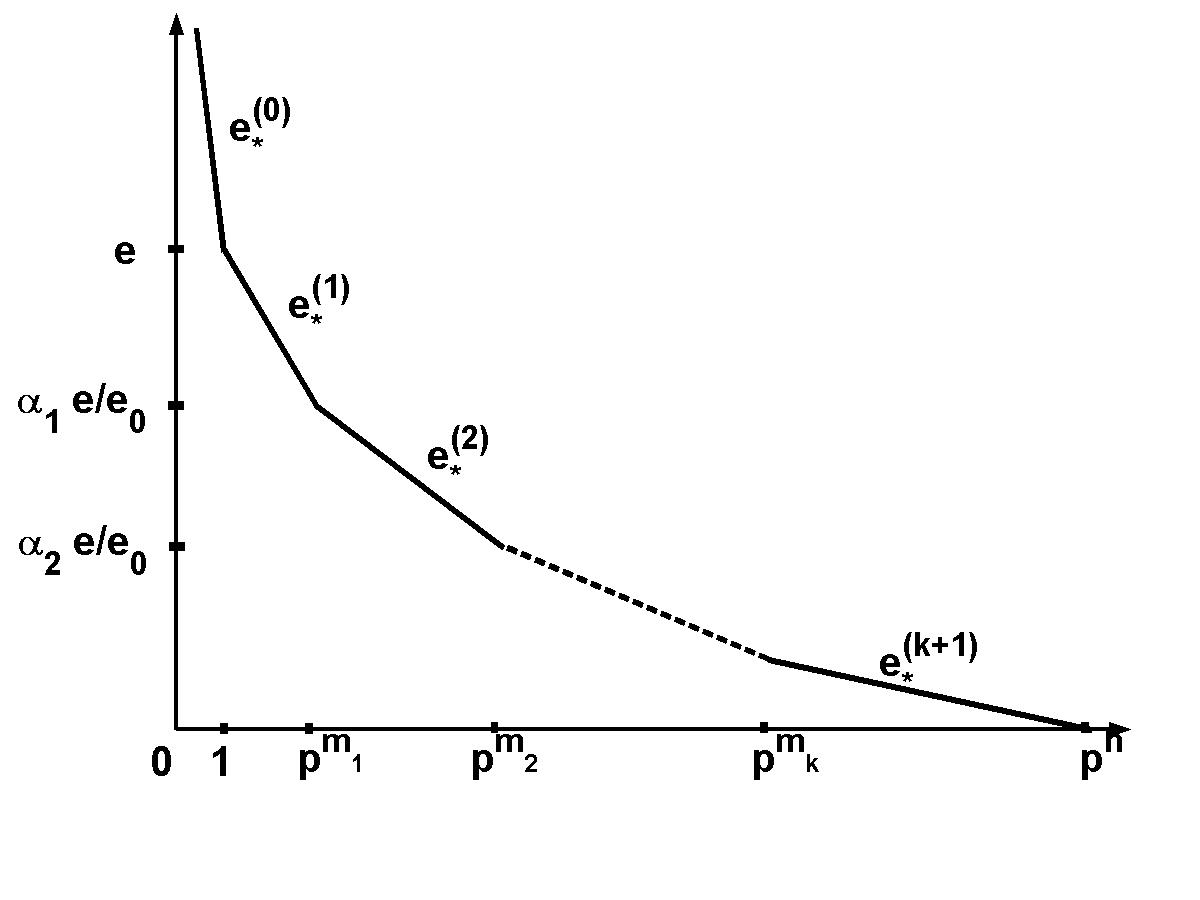
\includegraphics[height=5cm]{NewtonPolygon}
	\label{fig:Polygon}
\end{figure}

Обозначим через $e_*^{(i)}$ тангенс угла наклона прямой, соединяющей точки $(p^{m_i},\val(a_{p^{m_i}}))$ и $(p^{m_{i-1}},\val(a_{p^{m_{i-1}}}))$:
$$e_*^{(i)}:={e\over e_0}{\alpha_{i-1}-\alpha_{i}\over p^{m_i}-p^{m_{i-1}}}.$$
Числа $p^{m_i}$ и $e_*^{(i)}$ являются важными инвариантами формальной\linebreak группы $F$ (см. \cite{book4}).

В работе \cite{book2} доказано, что, если $e_0<p$, то $e_*^{(1)}>e_*^{(2)}>\dots>e_*^{(k+1)}$. Более того, верно следующее утверждение (см. лемму 2 в \cite{book2}).
\begin{proposition}
Пусть $z$ --- ненулевой корень изогении $[p]_F(X)$ в поле $L$. Тогда
$$\val(z)=e_*^{(i)}$$
при некотором $i:\ 1\Leq i\Leq k+1$, если $h\Geq2$. Если же $h=1$, то
$$\val(z)={e\over p-1}.$$
\end{proposition}
Аналогичные обозначания будут для других полей:\\
$T_K$ --- подполе инерции поля $K$ (максимальное неразветвлённое подполе в расширение $K/\Qp$), простым элементом в $T_K$ будет $p$.\\
$\OTK$ --- его кольцо целых.\\
$L$ --- нормальное расширение поля $K$.\\
$\OL$, $\ML$ --- кольцо целых поля $L$ и его максимальный идеал.\\
$\Pi$ --- простой элемент поля $L$.\\
$e=e(L/\Qp)$ --- абсолютный индекс ветвления поля $L$. Мы считаем, что $L/K$ не имеет высшего ветвления, то есть $(e,p)=1$.\\
$\val = \val_L$ --- нормирование в поле $L$.\\
$T_L$, $\OTL$ --- подполе инерции поля $L$ и его кольцо целых.\\
$\RL$ --- представители Тейхмюллера в поле $L$.\\
$G=Gal(L/K)$ --- группа Галуа расширения $L/K$.

\paragraph{}

Пусть $L/K$ --- нормальное расширение без высшего ветвления с группой Галуа $G=Gal(L/K)$. Тогда так же, как в работе \cite{VostokovLutzSimple}, сделаем $\OTK[G]$-модуль из $\OTL[X]$.  В поле $L$ всегда можно выбрать такой простой элемент $\Pi$, что элемент
$$\varepsilon_\sigma={\Pi^\sigma\over\Pi}\in\RL$$
является корнем из единицы степени взаимно простой с $p$ для любого автоморфизма $\sigma \in G$.

Теперь в кольце многочленов $\OTL[X]$ можно задать действие операторов из группы $G$, положив
$$X^\sigma=\varepsilon_\sigma X, \sigma\in G.$$
Тем самым кольцо $\OTL[X]$ становится модулем над групповым кольцом $\OTK[G]$.

Рассмотрим $\OTK[G]$-подмодуль $A_I$ из $\OTL[X]$ с $\OTK$-образующи\-ми $X^i$, где $I$ --- некоторая полная система вычетов по модулю $e\over e_0$. Тогда, в соответствии с леммой 3 работы \cite{VostokovLutzSimple} имеем следующее предложение.
\begin{proposition}
Пусть $L/K$ --- нормальное расширение без высшего ветвления. Тогда $\OTK[G]$-модуль $A_I$ является свободным \linebreak $\OTK[G]$-модулем ранга 1.
\end{proposition}

\section{Образующие модуля $F(\ML)$}
Рассмотрим формальный $\mathbb{Z}_p$-модуль $F(\ML)$, который как множество совпадает с максимальным идеалом $\ML$ кольца целых поля $L$. Структуру $\mathbb{Z}_p$-модуля на $F(\ML)$ зададим с помощью формального группового закона $F$:
$$\forall\alpha,\beta\in F(\ML) \quad \alpha+_F\beta:=F(\alpha,\beta),$$
$$\forall\alpha\in F(\ML), a\in\mathbb{Z}_p \quad a\alpha:=[a]_F(\alpha).$$
Тогда, если $e_0=e(K/\Qp)<p$, то, согласно работе \cite{book2}, получим следующие сравнения для элемента $\alpha\in F(\ML)$.
$$[p]_F(\alpha)\equiv
  \begin{cases}
  c_h(0)\alpha^{p^h}\mod\Pi^{p^h\val(\alpha)+1},& 1\Leq\val(\alpha)<e_*^{(k+1)} \cr
  \pi^{\alpha_i}c_i(0)\alpha^{p^{m_i}}\mod\Pi^{\alpha_i{e\over e_0}+p^{m_i}\val(\alpha)+1},&
  \begin{array}{c} e_*^{(i+1)}<\val(\alpha)<e_*^{(i)} \\ 1\Leq i\Leq k \\ \end{array}\cr
  pc_0(0)\alpha\mod\Pi^{e+\val(\alpha)+1},& e_*^{(1)}<\val(\alpha) \cr  \pi^{\alpha_{i-1}}c_{i-1}(0)\alpha^{p^{m_{i-1}}}\thickspace+\thickspace\pi^{\alpha_{i}}c_{i}(0)\alpha^{p^{m_{i}}}&\text{mod}\thickspace\Pi^{\alpha_{i}{e\over e_0}+e_*^{(i)}p^{m_{i}}+1},\cr 
  &\begin{array}{c} \val(\alpha)=e_*^{(i)} \\ 1\Leq i\Leq k+1\\ \end{array} \cr
  \end{cases}
$$

С помощью этих сравнений можно получить образующие для формального модуля $F(\ML)$. Пусть $\theta$ из $\RL$, тогда с помощью $\varepsilon_s(\theta)$ сопоставим $\theta$ некий элемент из $F(\ML)$ такой, что\linebreak $\varepsilon_s(\theta)\equiv\theta\Pi^s\mod\Pi^{s+1}$.
\begin{proposition}
Любой элемент $\alpha\in F(\ML)$ представим в виде суммы
$$\alpha={\sum}_{(F)}^*[p]_F^r\varepsilon_s(\theta_{s,r}),$$
где символ $\sum_{(F)}^*$ обозначает суммирование по всем неотрицательным $r$ и по индексам $s$ из некоторого специального индексного множества $I$. При этом, если поле $L$ не содержит нетривиальных корней изогении $[p]_F$, то такое представление однозначно.
\end{proposition}
В частности, в множестве $I$ не будут встречаться индексы, большие $e_*^{(1)}+e$. Запишем $I$ в виде $I=\{1\Leq s\Leq e_*^{(1)}+e\ |\ \bigstar\}$, где $\bigstar$ --- некое условие, которое мы получим ниже.
\begin{proof}
Для начала индукцией проверим, что любой элемент $\alpha$ из $F(\ML)$ можно представить в виде суммы следующего вида: $\alpha={\sum\limits_{s=1}^\infty}_{(F)}\varepsilon_s(\theta_s)$, где $\theta_s\in\RL,\ \varepsilon_s(\theta_s)\in F(\ML)$ такие, что $\varepsilon_s(\theta_s)\equiv\theta\Pi^s\mod\Pi^{s+1}$.

База индукции очевидна, так как любой элемент из $F(\ML)$ имеет вид $\alpha=\theta_1\Pi+\dots\ \Rightarrow \alpha\equiv\theta_1\Pi\mod\Pi^2$.

Пусть теперь $\alpha\equiv{\sum\limits_{s=1}^t}_{(F)}\varepsilon_s(\theta_s)\mod\Pi^{t+1} \Rightarrow \alpha={\sum\limits_{s=1}^t}_{(F)}\varepsilon_s(\theta_s) +\linebreak+\ \theta_{t+1}\Pi^{t+1}+\dots \equiv {\sum\limits_{s=1}^t}_{(F)}\varepsilon_s(\theta_s) + \theta_{s+1}\Pi^{t+1}\mod\Pi^{t+2}\equiv {\sum\limits_{s=1}^t}_{(F)}\varepsilon_s(\theta_s) +_{F}\linebreak+_{F}\ \theta_{s+1}\Pi^{t+1}\mod\Pi^{t+2}$.

Таким образом, мы получили, что для каждого $t>0\linebreak \alpha\equiv{\sum\limits_{s=1}^t}_{(F)}\varepsilon_s(\theta_s)\mod\Pi^{t+1}$, а значит $\alpha={\sum\limits_{s=1}^\infty}_{(F)}\varepsilon_s(\theta_s)$.

Далее, пользуясь сравнениями, уберём лишние индексы в этой сумме. Будем считать, что $\beta=\theta\Pi^{\val(\beta)}+\dots\in F(\ML),\linebreak c_i(0)=c_i+\dots,\ \pi=\xi\Pi^{e\over e_0}+\dots,\ p=\zeta\Pi^e+\dots$, где $\theta,c_i,\xi,\zeta\in\RL$.

\begin{enumerate}
\item Если $s=\val(\beta)>e_*^{(1)}$, то $[p]_F(\beta)=pc_0(0)\beta+\dots\equiv\linebreak\equiv\zeta c_0\theta\Pi^{s+e}\mod\Pi^{s+e+1}$, следовательно, если в качестве $\theta$\linebreak взять $\theta=\theta_{s+e}(\zeta c_0)^{-1}\in\RL$, то $\beta\equiv\theta\Pi^{s}\mod\Pi^{s+1}\equiv\linebreak\equiv\varepsilon_{s}(\theta)\mod\Pi^{s+1}$, а для слагаемого с индексом $s+e$ получим следующее сравнение:
$$\varepsilon_{s+e}(\theta_{s+e})\equiv[p]_F(\beta)\mod\Pi^{s+e+1}\equiv[p]_F(\varepsilon_s(\theta))\mod\Pi^{s+e+1}.$$
Это сравнение означает, что в сумме $\alpha={\sum\limits_{s=1}^\infty}_{(F)}\varepsilon_s(\theta_s)$ любое слагаемое $\varepsilon_j(\theta_j)$ индекса $j>e_*^{(1)}+e$ можно заменить на слагаемое вида $[p]_F(\varepsilon_{j-e}(\theta_{j-e,1}))$, то есть в индексном множестве $I$ нет индексов, больших $e_*^{(1)}+e$.
\item Если $1\Leq s=\val(\beta)<e_*^{(k+1)}$, то $[p]_F(\beta)\equiv c_h\theta^{p^h}\Pi^{p^hs}\mod\Pi^{p^hs+1}$. Представители Тейхмюллера $\RL\ p$-делимы, значит $\theta=\linebreak=(c_h^{-1}\theta_{p^hs})^{1\over p^h}$ будет лежать в $\RL$. При таком $\theta$ получим, что
$$[p]_F(\varepsilon_s(\theta))\equiv[p]_F(\beta)\mod\Pi^{p^hs+1}\equiv\theta_{p^hs}\Pi^{p^hs}\mod\Pi^{p^hs+1}.$$
А это означает, что в сумме $\alpha={\sum\limits_{s=1}^\infty}_{(F)}\varepsilon_s(\theta_s)$ будут отсутствовать слагаемые вида $\varepsilon_{p^hs}(\theta_{p^hs})$, где $1\Leq s<e_*^{(k+1)}$.
\item Если $e_*^{(i+1)}<s=\val(\beta)<e_*^{(i)}$ для некоторого $1\Leq i\Leq k$, то
$$[p]_F(\varepsilon_s(\theta))\equiv[p]_F(\beta)\mod\Pi^{\alpha_i{e\over e_0}+p^{m_i}s+1}\equiv$$
$$\equiv\xi^{\alpha_i}c_i\theta^{p^{m_i}}\Pi^{\alpha_i{e\over e_0}+p^{m_i}s}\mod\Pi^{\alpha_i{e\over e_0}+p^{m_i}s+1}.$$
$\xi^{\alpha_i}c_i\theta^{p^{m_i}s}\in\RL$, поэтому мы можем рассмотреть $\theta=\linebreak=(\xi^{-\alpha_i}c_i^{-1}\theta_{\alpha_i{e\over e_0}+p^{m_i}s})^{1\over p^{m_i}}\in\RL$. Тогда получим, что для любого индекса $j=\alpha_i{e\over e_0}+p^{m_i}s$ при некотором $1\Leq i\Leq k$ и $e_*^{(i+1)}<s<e_*^{(i)}$ будет выполняться сравнение
$$[p]_F(\varepsilon_s(\theta))\equiv\varepsilon_j(\theta_j)\mod\Pi^{j+1},$$
а значит из индексного множества $I$ можно убрать все такие индексы $j$.
\item В случае, если $s=\val(\beta)=e_*^{(i)}$ для некоторого $1\Leq i\Leq k+1$, рассмотрим $j=\alpha_i{e\over e_0}+p^{m_i}s$, тогда
$$[p]_F(\varepsilon_s(\theta))\equiv[p]_F(\beta)\mod\Pi^{j+1}\equiv$$
$$\equiv(\xi^{\alpha_{i-1}}c_{i-1}\theta^{p^{m_{i-1}}}+\xi^{\alpha_i}c_i\theta^{p^{m_i}})\Pi^j\mod\Pi^{j+1}.$$
Будем считать, что сравнения
$$\theta_j\equiv \xi^{\alpha_{i-1}}c_{i-1}\theta^{p^{m_{i-1}}}+\xi^{\alpha_i}c_i\theta^{p^{m_i}}\mod\Pi$$
имеют решения $\theta$ в $\RL$ для любого $\theta_j$ из $\RL$, тогда индексы вида $e_*^{(i)}$, где $1\Leq i\Leq k+1$, можно выкинуть из множества $I$.

\end{enumerate}
Таким образом, условие $\bigstar$ состоит из четырёх пунктов:
\begin{enumerate}
\item $s\Leq e+e_*^{(1)}=\alpha_0{e\over e_0}+p^{m_0}e_*^{(1)}$,
\item $s\neq p^hj=\alpha_{k+1}{e\over e_0}+p^{m_{k+1}}j$ ни для какого $1\Leq j< e_*^{(k+1)}$,
\item $s\neq\alpha_i{e\over e_0}+p^{m_i}j$ ни для каких $1\Leq i\Leq k$ и $e_*^{(i+1)}<j<e_*^{(i)}$,
\item $s\neq\alpha_i{e\over e_0}+p^{m_i}e_*^{(i)}$ ни для какого $1\Leq i\Leq k+1$.
\end{enumerate}
В итоге любой элемент $\alpha$ из $F(\ML)$ можно представить в виде суммы $\alpha=\sum_{(F)}^*[p]_F^r\varepsilon_s(\theta_{s,r})$, где символ $\sum_{(F)}^*$ означает, что суммирование ведётся по всем неотрицательным $r$, а $s$ берутся из индексного множества $I=\{1\Leq s\Leq e+e_*^{(1)}\ |\ \bigstar\}$.

Ясно, что, если $L$ не содержит нетривиальных корней изогении $[p]_F$, то такое представление будет однозначным.
\end{proof}

\paragraph{}

Разобьём индексное множество $I$ на непересекающиеся подмножества так, чтобы в каждом из них было по $e\over e_0$ различных представителей вычетов по модулю $e\over e_0$. Рассмотрим числа $i_j:=\alpha_j{e\over e_0}+\linebreak+p^{m_j}e_*^{(j+1)},\ 0\Leq j\Leq k+1$ (здесь и в дальнейшем будем считать, что $e_*^{(k+2)}=0$), тогда $I$ представляется в виде объединения непересекающихся множеств $I_j:=\{i_j\Leq s<i_{j-1}\ |\ \bigstar\}$: $I=\bigcup\limits_{j=1}^{k+1}I_j$. Заметим, что для каждого $j$ все индексы $s=\alpha_j{e\over e_0}+p^{m_j}l$, где $e_*^{(j+1)}<l<e_*^{(j)}$, лежат в интервале $I_j$. Действительно:
$$s=\alpha_j{e\over e_0}+p^{m_j}l>\alpha_j{e\over e_0}+p^{m_j}e_*^{(j+1)}=i_j,$$ 
$$s=\alpha_j{e\over e_0}+p^{m_j}l<\alpha_j{e\over e_0}+p^{m_j}e_*^{(j)}=\alpha_j{e\over e_0}+p^{m_j}{e\over e_0}{\alpha_{j-1}-\alpha_j\over p^{m_j}-p^{m_{j-1}}}=$$
$$={e\over e_0}{p^{m_j}\alpha_j-p^{m_{j-1}}\alpha_j+p^{m_j}\alpha_{j-1}-p^{m_j}\alpha_j\over p^{m_j}-p^{m_{j-1}}}={e\over e_0}{p^{m_j}\alpha_{j-1}-p^{m_{j-1}}\alpha_j\over p^{m_j}-p^{m_{j-1}}}=$$
$$={e\over e_0}{p^{m_j}\alpha_{j-1}-p^{m_{j-1}}\alpha_{j-1}+p^{m_{j-1}}\alpha_{j-1}-p^{m_{j-1}}\alpha_j\over p^{m_j}-p^{m_{j-1}}}=$$
$$=\alpha_{j-1}{e\over e_0}+p^{m_{j-1}}{e\over e_0}{\alpha_{j-1}-\alpha_j\over p^{m_j}-p^{m_{j-1}}}=\alpha_{j-1}{e\over e_0}+p^{m_{j-1}}e_*^{(j)}=i_{j-1}.$$
Таким образом, условие $\bigstar$ в каждом из множеств $I_j$ будет равномерно <<выкалывать>> индексы с шагом $p^{m_j}$. Из каждого $I_j$ будет <<выколото>> ровно $e_*^{(j)}-e_*^{(j+1)}$ индексов, а значит из всех $e+e_*^{(1)}$ индексов в множестве $I$ будет <<выколото>> ровно $(e_*^{(k+1)}-e_*^{(k+2)})+(e_*^{(k)}-\linebreak-\ e_*^{(k+1)})+\dots+(e_*^{(1)}-e_*^{(2)})=e_*^{(1)}$ индексов, а значит в $I$ останется $e$ индексов. Разобьём их на на $e_0$ групп по $e\over e_0$ в каждой.  Ясно, что если для любого $j\quad {e\over e_0}$ делит $(p^{m_j}-1):\ t_j{e\over e_0}=p^{m_j}-1$, то каждое из множеств $I_j$ разбивается в объединение $t_j(e_*^{(j)}-e_*^{(j+1)})$ множеств по $e\over e_0$ представителей вычетов по модулю $e\over e_0$.  Следовательно можно будет наше множество $I$ представить в виде объединения $I=\bigcup\limits_{i=1}^{e_0}I_{e\over e_0}^i$, где множества $I_{e\over e_0}^i$ имеют такой вид, как требуется в предложении 1.

\paragraph{}

Используя результаты этого параграфа, получим, что\linebreak $\OTK[G]$-модуль $A_I$, построенный на $\OTK[X]$ образующих $X^s$, где $s$ из нашего индексного множества $I=\{1\Leq s\Leq e+e_*^{(1)}\ |\ \bigstar\}$ будет представляться в виде прямой суммы модулей $A_{I_{e\over e_0}^i}$: $A_I=\bigoplus\limits_{i=1}^{e_0}A_{I_{e\over e_0}^i}$. В предложении 2 говорится, что каждый модуль $A_{I_{e\over e_0}^i}$ является свободным $\OTK[G]$-модулем ранга $1$, а значит будет верным следующее предложение.

\begin{proposition}
Пусть $I=\{1\Leq s\Leq e+e_*^{(1)}\ |\ \bigstar\}$. Рассмотрим $\OTK[G]$-модуль $A_I$, с $\OTK$-образующими $X^s$, где $s\in I$. Тогда $A_I$ является свободным $\OTK[G]$-модулем ранга $e_0$.
\end{proposition}


\section{Итоговый результат}

\paragraph{}

Рассмотрим $\OTK[G]$-модуль $A_I$, который по предложению 4 является свободным $\OTK[G]$-модулем ранга $e_0$. Пусть $\beta_l,\beta_2,\dots,\beta_{e_0}$ образуют нормальный базис модуля $A_I$, то есть элементы\linebreak $\{\beta_l^\sigma\ |\ 1\Leq l\Leq e_0,\sigma\in G\}$ образуют базис модуля $A_I$ над $\OTK$. Тогда, если $b_1,b_2,\dots,b_n\in\OTK$ образуют базис кольца $\OTK$ над $\Zp$, то множество $\{b_j\beta_l\ |\ 1\Leq l\Leq e_0, 1\Leq j\Leq n\}$ является нормальным базисом модуля $A_I$ как $\Zp[G]$-модуля, а это означает, что $A_I$ является свободным $\Zp[G]$-модулем ранга $ne_0$, где $n=(\OTK:\Zp)$.

В предложении 3 говорилось, что любой $\alpha$ из $F(\ML)$ представим в виде $\alpha=\sum_{(F)}^*[p]^r_F\varepsilon_s(\theta_{s,r})$, где $\varepsilon_s(\theta_{s,r})\equiv\theta_{s,r}\Pi^{s}\mod\Pi^{s+1}$. Из свойств функции $E_F$ ясно, что $\varepsilon_s(\theta_{s,r})\equiv E_F(\theta_{s,r}X^s)|_{X=\Pi}\mod\Pi^{s+1}$, а значит
$$\forall\alpha\in F(\ML)\quad \alpha=E_F({\sum\limits_{s\in I\ r\Geq0}}p^r\theta_{s,r}X^s)|_{X=\Pi}=E_F(\varphi)|_{X=\Pi},$$
где $\varphi$ из $A_I$. Так как $E_F(\varphi+\psi)=E_F(\varphi)+_FE_F(\psi)$, то получаем, что функция $E_F$ задаёт гомоморфизм $\Zp$-модулей $A_I$ и $F(\ML)$. Если поле $L$ не содержит нетривиальных корней изогении $[p]_F$, то $E_F$, по предложению 3, будет $\Zp$-изоморфизмом. Более того, по свойству 3, $E_F(X^\sigma)=(E_F(X))^\sigma$ для любого $\sigma$ из группы Галуа $G$, а значит $E_F$ задаёт изоморфизм $A_I$ и $F(\ML)$ как $\Zp[G]$-модулей.

Рассмотрим образующие $\Zp[G]$-модуля $A_I:$
$$\{b_j\beta_l\ |\ 1\Leq l\Leq e_0, 1\Leq j\Leq n\}.$$
Отображение $E_F$ будет переводить их в образующие $\Zp[G]$-модуля $F(\ML)$, а это значит, что $F(\ML)$ является свободным $\Zp[G]$-модулем ранга $ne_0$.

Аналогичные рассуждения можно провести и для остальных модулей $F(\ML^i)$ фильтрации Лютц.

\paragraph{}
В итоге, мы получили следующий результат.
\begin{theorem}
Пусть $K$ --- конечное расширение поля $\Qp$, с индексом ветвления $e_0=e(K/\Qp)<p$, и пусть $L/K$ --- нормальное расширение без высшего ветвления с группой Галуа $G=Gal(L/K)$. Рассмотрим формальную группу $F(X,Y)$ конечной высоты $h$, заданную над кольцом целых $\OK$ поля $K$. Пусть $[p]_F(X)=pc_0(X)X+\pi^{\alpha_1}c_1(X)X^{p_{m_1}}+\dots+\pi^{\alpha_k}c_kX^{p^{m_k}}+c_h(X)X^{p^h}$ --- эндоморфизм умножения на $p$ формальной группы $F$. Тогда, если выполняются следующие условия:
\begin{enumerate}
\item $L$ не содержит нетривиальных корней изогении $[p]_F$,
\item Для любого $i$ из $\{1,2,\dots,k+1\}$ сравнение $\theta_*\equiv\xi^{\alpha_{i-1}}c_{i-1}\theta^{p^{m_{i-1}}}+\xi^{\alpha_{i}}c_{i}\theta^{p^{m_{i}}}\mod\Pi$ имеет решение $\theta\in\RL$ для любого $\theta_*\in\RL$, где $\pi=\xi\Pi^{e\over e_0}+\dots$,
\end{enumerate}
то $F(\ML)$ является свободным $\Zp[G]$-модулем ранга $ne_0$, где $n=(\OTK:\Zp)$. Аналогичный результат верен и для $F(\ML^i)$.
\end{theorem}

\pagebreak

\section{Обозначения}
\paragraph{}
В данной работе будем рассматривать многомерное локальное поле $K=k^{(n)}, k^{(n-1)},\dots$ $,k^{(1)},k^{(0)}=\Fq,$ в случае, когда $k^{(1)} = k$ --- одномерное локальное поле характеристики ноль (конечное расширение $\Qp$). В этом случае $K = k((t_2))\dots((t_n))$, где набор $t_n,\dots,t_1$ --- система локальных параметров поля $K$. Таким образом, $t_i$ является единицей в полях $K,k^{(n-1)},\dots,k^{(i+1)}$ и при этом в поле $k^{(i)}$ является простым элементом. Для всех $0 \Leq i < n$ поле $k^{(i)}$ является полем вычетов для полного дискретно нормированного поля $k^{(i+1)}$. Через $\pi = t_n$ будем обозначать простой элемент поля $k^{(n)}$, а $\val_{k^{(i)}}$ --- нормирование в поле $k^{(i)}$.\\
$\overline{\val_K}=\olval=(\val_1,\dots,\val_n):K^*\rightarrow\Z^n$ --- нормирование ранга $n$ в $K$. Здесь $\val_n(a)=\val_{k^{(n)}}(a)$, а для $1\Leq i<n$
$$v_i(a) = \val_{k^{(i)}} \left( \overline {a \over { t_n^{\val_n(a)} \ldots t_{i+1}^{\val_{i+1}(a)} } } \right),$$\\
$\Z^n$ считается лексикографически упорядоченным.\\
$\OK=\{a\in K^*\ |\ \overline{\val}(a)\Geq0\}$ --- кольцо нормирования, которое не зависит от выбора системы локальных параметров.\\
$\MK=\mathfrak{M}=\{a\in\OK\ |\ \overline{\val}(a)>0\}$ --- максимальный идеал кольца нормирования.\\
$\overline{K} = \OK/\MK$ --- поле вычетов $K$ относительно $\olval$ будет иметь характеристику $p$, так как $\olval(p) > (0,\ldots,0)$, а значит $p\in \MK$ и $p \equiv 0 \mod \MK$.\\
Далее, $e_K$ --- индекс ветвления поля $K$ относительно нормирования $\val=\val_n$, то есть $\val(p)=e_K$.\\
$\overline{e_K}$ --- индекс ветвления поля $K$ относительно нормирования $\olval$.\\

Пусть $L/K$ --- нормальное расширение без высшего ветвления с группой Галуа $G=Gal(L/K)$, тогда $L = L^{(1)}((T_2))\dots((T_n)),$ где $L^{(1)}$ --- конечное расширение поля $k$. При этом обозначим через $(\Pi = T_1, T_2, \dots, T_n)$ --- систему локальных параметров в поле $L$.
$\OL,\ML$ --- кольцо целых поля $L$ и его максимальный идеал, а $\overline{e}=(e_1, e_2, \ldots, e_n)$ абсолютный индекс вевтения поля $L$ относительно нормирования $\overline{\val_L} = (\val_1^L, \ldots, \val_n^L)$, полученного продолжением нормирования $\olval$ с поля $K$ на поле $L$. $\RL$ --- мультипликативная система представителей Тейхмюллера поля $L^{(0)}$, где $L_0$ --- подполе инерции в расширении $L_1/\Qp$.\\
Также, нам могут понадобиться $\Ok$ и $\OLO$ --- кольца целых одномерных локальных полей $k$ и $L^{(1)}$ соответственно, и их максимальные идеалы: $\Mk$ и $\MLO$.


Возьмём $F(X,Y)\in\OK[X,Y]$ --- формальный групповой закон, определяющий одномерную формальную группу конечной высоты $h$.\\ 
Рассмотрим максимальный идеал кольца целых поля $L$ и его степени $\ML\supset\ML^2\supset\dots$, с помощью группового закона $F(X,Y)$ на этих идеалах можно задать структуру формальных $\Zp$-модулей. $F(\ML^i)$ совпадает с $\ML^i$ как множество. Определим на нём операцию сложения через $F(X,Y)$: $\forall\alpha,\beta\in\ML^i:\ \alpha+_F\beta=F(\alpha,\beta).$ Кольцо $\Zp$ вкладывается в кольцо эндоморфизмов формальной группы $F$ (\cite[\S 2]{book6} --- это вложение $End(F)$ в $\OK$, но существует некое кольцо $\mathfrak{O}_0$, изоморфное образу $End(F)$ в $\OK$; а это $\mathfrak{O}_0$ содержит $\Zp$ \cite[\S2.3]{book6}), поэтому для любого скаляра $a\in\Zp$ и любого $\alpha\in\ML^i$ естественным образом определяется умножения на скаляр: $a\alpha=[a]_F(\alpha)$.\\
Коэффиценты группового закона $F \in \OK[X,Y]$ неподвижны относительно действия группы $G$, поэтому модули $F(\ML^i)$ можно рассматривать как $\Zp[G]$-модули. Таким образом мы получили филтрацию Лютц модулей Галуа: $F(\ML) \supset F(\ML^2) \supset F(\ML^3) \supset \ldots$, для которых в данной работе явным образом будут построены образующие.

\section{Образующие модуля $F(\ML)$}

Возьмём $[p]_F(X) \in pX+\OK[[X]]X^2$ --- эндоморфизм умножения на $p$ формальной группы $F$. В работе \cite[Арифметика формального модуля]{book2} получены образующие $F(\ML)$ как $\Zp$-модуля для случая одномерной формальной группы $F$ конечной высоты $h$, заданной над кольцом целых локального поля $K$ с абсолютным индексом ветвления $e_K \Leq p$. Этот результат может быть применён в расширении многомерных полей $L/K$. Применим его в нашем случае.\\

Через $e_K$ и $e_L = e_n$ мы обозначаем абсолютные индексы ветвления поле $K$ и $L$ относительно нормирования $\val$. \\
В соответствии с работой \cite{book2} эндоморфизм $[p]_F(X)$ можно записать в виде
$$[p]_F(X)=pc_0(X)X+\pi^{\alpha_1}c_1(X)X^{p^{m_1}}+\dots+\pi^{\alpha_k}c_k(X)X^{p^{m_k}}+c_h(X)X^{p^h},$$
где $c_i(X) \in \OK[[X]]^*$, $c_0(X) \equiv 1 \mod X$, $\alpha_0:=e_K>\alpha_1>\alpha_2>\dots>\alpha_k>\alpha_{k+1}:=0$, $0=m_0<m_1<m_2<\dots<m_k<m_{k+1}:=h$.

Для $[p]_F(X)$ можно построить многоугольник Ньютона. В области $M=\{(x,y)\in\Rb^2\ |\ x\Geq0,y\Geq0\}$ отметим точки $(i,\val(a_i))$, где $ 1\Leq i\Leq p^h$. Из всех ломаных с вершинами в отмеченных точках и соединяющих точки $(1,\val(a_1))$ и $(p^h,\val(a_{p^h}))$ выберем наиболее близкую к границе области $M$. Эта ломаная является нижней границей выпуклой оболочки множества $\{i,\val(a_i)\ |\ 1\Leq i\Leq p^h\}$. Постороенная ломаная будет многоугольником 
\begin{figure}[h]
	\centering	
	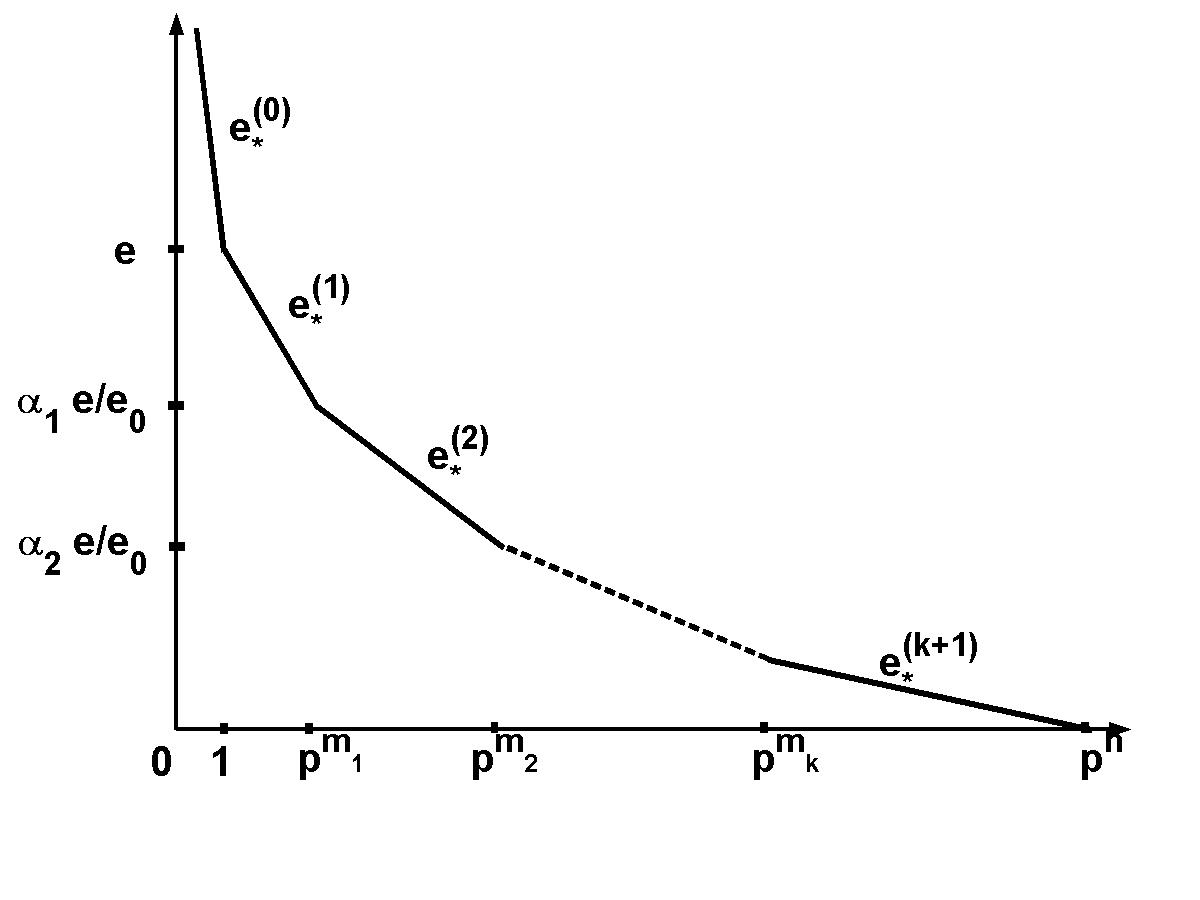
\includegraphics[height=5cm]{NewtonPolygon}
	\label{fig:Polygon}
	\caption{Многоугольник Ньютона для $[p]_F$}
\end{figure}

Обозначим через $e_*^{(i)}$ тангенс угла наклона прямой, соединяющей точки $(p^{m_i},\val(a_{p^{m_i}}))$ и $(p^{m_{i-1}},\val(a_{p^{m_{i-1}}}))$:
$$e_*^{(i)}:={e_L\over e_K}{\alpha_{i-1}-\alpha_{i}\over p^{m_i}-p^{m_{i-1}}}.$$
Числа $p^{m_i}$ и $e_*^{(i)}$ являются важными инвариантами формальной группы $F$ (см. \cite{book4}).

В работе \cite{book2} доказано, что, если $e_K \Leq p$, то $e_*^{(1)}>e_*^{(2)}>\dots>e_*^{(k+1)}$. Более того, верно следующее утверждение \cite[Лемма 2]{book2}).
\begin{proposition}
	Пусть $z$ --- ненулевой корень изогении $[p]_F(X)$ в поле $L$. Если $h \Geq 2$, тогда $\val(z)=e_*^{(i)}$ при некотором $i:\ 1\Leq i\Leq k+1$. Если же $h=1$, то $\val(z)={e_L\over p-1}$.
\end{proposition}

Кроме того, из представления изогении через вышеприведённые инварианты получаем сравнения для произвольного элемента $\alpha\in F(\ML)$:
$$[p]_F(\alpha)\equiv
\begin{cases}
c_h\alpha^{p^h}\mod\Pi^{p^h\val(\alpha)+1},& 1\Leq\val(\alpha)<e_*^{(k+1)} \cr
\pi^{\alpha_i}c_i\alpha^{p^{m_i}}\mod\Pi^{\alpha_i{e_L \over e_K}+p^{m_i}\val(\alpha)+1},&
e_*^{(i+1)}<\val(\alpha)<e_*^{(i)}, 1 \Leq i \Leq k \cr
pc_0\alpha\mod\Pi^{e_L+\val(\alpha)+1},& e_*^{(1)}<\val(\alpha) \cr  \pi^{\alpha_{i-1}}c_{i-1}\alpha^{p^{m_{i-1}}}\thickspace+\thickspace\pi^{\alpha_{i}}c_{i}\alpha^{p^{m_{i}}}\text{mod}\thickspace\Pi^{\alpha_{i}{e_L \over e_K}+e_*^{(i)}p^{m_{i}}+1}, 
& \val(\alpha)=e_*^{(i)}, 1\Leq i\Leq k+1 \cr
\end{cases}
$$\\
Под $\val=\val_L$ понимается нормирование на $n$-ой компоненте многомерного поля $L$, а $c_{i} = c_{i}(0)$ --- значения соответствующих многочленов в нуле.

С помощью этих сравнений получим образующие для формального модуля $F(\ML)$ как $\Zp$-модуля. Пусть $\theta$ из $\RL$, тогда с помощью $\varepsilon_s(\theta)$ сопоставим $\theta$ некий элемент из $F(\ML)$ такой, что $\varepsilon_s(\theta)\equiv\theta\Pi^s\mod\Pi^{s+1}$. 
Для начала индукцией проверим, что любой элемент $\alpha$ из $F(\ML)$ можно представить в виде суммы следующего вида: $\alpha={\sum\limits_{s=1}^\infty}_{(F)}\varepsilon_s(\theta_s)$, где $\theta_s\in\RL$, $\varepsilon_s(\theta_s)\in F(\ML)$ такие, что $\varepsilon_s(\theta_s)\equiv\theta\Pi^s\mod\Pi^{s+1}$.\\
База индукции очевидна, так как любой элемент из $F(\ML)$ имеет вид $\alpha=\theta_1\Pi+\dots\ \Rightarrow \alpha\equiv\theta_1\Pi\mod\Pi^2$.\\
Пусть теперь $\alpha\equiv{\sum\limits_{s=1}^t}_{(F)}\varepsilon_s(\theta_s)\mod\Pi^{t+1}$, тогда $\alpha={\sum\limits_{s=1}^t}_{(F)}\varepsilon_s(\theta_s) +\ \theta_{t+1}\Pi^{t+1}+\dots \equiv {\sum\limits_{s=1}^t}_{(F)}\varepsilon_s(\theta_s) + \theta_{s+1}\Pi^{t+1}\mod\Pi^{t+2}\equiv {\sum\limits_{s=1}^t}_{(F)}\varepsilon_s(\theta_s) +_{F}\ \theta_{s+1}\Pi^{t+1}\mod\Pi^{t+2}$.
Таким образом, мы получили, что для каждого $t>0$ выполняется сравнение $\alpha\equiv{\sum\limits_{s=1}^t}_{(F)}\varepsilon_s(\theta_s)\mod\Pi^{t+1}$, а значит $\alpha={\sum\limits_{s=1}^\infty}_{(F)}\varepsilon_s(\theta_s)$. \\

Далее, пользуясь сравнениями, уберём лишние индексы в этой сумме. Будем считать, что $\beta=\theta\Pi^{\val(\beta)}+\dots\in F(\ML),\ c_i(0)=\gamma_i+\dots,\ \pi=\xi\Pi^{e_L\over e_K}+\dots,\ p=\zeta\Pi^e+\dots$, где $\theta,\gamma_i,\xi,\zeta\in\RL$.

\begin{enumerate}
	\item Если $s=\val(\beta)>e_*^{(1)}$, то $[p]_F(\beta)=pc_0(0)\beta+\dots\equiv\zeta \gamma_0\theta\Pi^{s+e_L}\mod\Pi^{s+e_L+1}$, следовательно, если в качестве $\theta$ взять $\theta=\theta_{s+e_L}(\zeta \gamma_0)^{-1}\in\RL$, то $\beta\equiv\theta\Pi^{s}\mod\Pi^{s+1}\equiv\varepsilon_{s}(\theta)\mod\Pi^{s+1}$, а для слагаемого с индексом $s+e_L$ получим следующее сравнение:
	$$\varepsilon_{s+e_L}(\theta_{s+e_L})\equiv[p]_F(\beta)\mod\Pi^{s+e_L+1}\equiv[p]_F(\varepsilon_s(\theta))\mod\Pi^{s+e_L+1}.$$
	Это сравнение означает, что в сумме $\alpha={\sum\limits_{s=1}^\infty}_{(F)}\varepsilon_s(\theta_s)$ любое слагаемое $\varepsilon_j(\theta_j)$ индекса $j>e_*^{(1)}+e_L$ можно заменить на слагаемое вида $[p]_F(\varepsilon_{j-e_L}(\theta_{j-e_L,1}))$, то есть в индексном множестве $I$ нет индексов, больших $e_*^{(1)}+e_L$. А значит элемент $\alpha \in F(\ML)$ можно представить в виде $\alpha = {\sum\limits_{s=1}^{e_*^{(1)} + e_L}}_{(F)}[p]_F^r(\varepsilon_s(\theta_{s,r}))$ по всем $r \Geq 0$.
	\item Если $1 \Leq s= \val(\beta) < e_*^{(k+1)}$, то $[p]_F(\beta) \equiv \gamma_h\theta^{p^h}\Pi^{p^hs}\mod\Pi^{p^hs+1}$. Представители Тейхмюллера $\RL\ p$-делимы, значит $\theta=(\gamma_h^{-1}\theta_{p^hs})^{1\over p^h}$ будет лежать в $\RL$. При таком $\theta$ получим, что
	$$[p]_F(\varepsilon_s(\theta))\equiv[p]_F(\beta)\mod\Pi^{p^hs+1}\equiv\theta_{p^hs}\Pi^{p^hs}\mod\Pi^{p^hs+1}.$$
	А это означает, что в сумме $\alpha={\sum\limits_{s=1}^{e_*^{(1)} + e_L}}_{(F)}[p]_F^r(\varepsilon_s(\theta_{s,r}))$ будут отсутствовать слагаемые вида $\varepsilon_{p^hs}(\theta_{p^hs,r})$, где $1 \Leq s < e_*^{(k+1)}$.
	\item Если $e_*^{(i+1)}<s=\val(\beta)<e_*^{(i)}$ для некоторого $1\Leq i\Leq k$, то
	$$[p]_F(\varepsilon_s(\theta))\equiv[p]_F(\beta)\mod\Pi^{\alpha_i{e_L \over e_K}+p^{m_i}s+1} \equiv \xi^{\alpha_i}\gamma_i\theta^{p^{m_i}}\Pi^{\alpha_i{e_L \over e_K}+p^{m_i}s}\mod\Pi^{\alpha_i{e_L\over e_K}+p^{m_i}s+1}.$$
	$\xi^{\alpha_i}\gamma_i\theta^{p^{m_i}s}\in\RL$, поэтому мы можем рассмотреть $\theta=(\xi^{-\alpha_i}\gamma_i^{-1}\theta_{\alpha_i{e_L \over e_K}+p^{m_i}s})^{1\over p^{m_i}}\in\RL$. Тогда получим, что для любого индекса $j=\alpha_i{e_L\over e_K}+p^{m_i}s$ при некотором $1\Leq i\Leq k$ и $e_*^{(i+1)}<s<e_*^{(i)}$ будет выполняться сравнение
	$$[p]_F(\varepsilon_s(\theta))\equiv\varepsilon_j(\theta_j)\mod\Pi^{j+1},$$
	а значит из индексного множества $I$ можно убрать все такие индексы $j$.
	\item В случае, если $s=\val(\beta)=e_*^{(i)}$ для некоторого $1\Leq i\Leq k+1$, рассмотрим $j=\alpha_i{e_L \over e_K}+p^{m_i}s$, тогда
	$$[p]_F(\varepsilon_s(\theta))\equiv[p]_F(\beta)\mod\Pi^{j+1} \equiv (\xi^{\alpha_{i-1}}\gamma_{i-1}\theta^{p^{m_{i-1}}}+\xi^{\alpha_i}\gamma_i\theta^{p^{m_i}})\Pi^j\mod\Pi^{j+1}.$$
	Будем считать, что сравнения
	$$\theta_j\equiv \xi^{\alpha_{i-1}}\gamma_{i-1}\theta^{p^{m_{i-1}}}+\xi^{\alpha_i}\gamma_i\theta^{p^{m_i}}\mod\Pi$$
	имеют решения $\theta$ в $\RL$ для любого $\theta_j$ из $\RL$, тогда индексы вида $e_*^{(i)}$, где $1\Leq i\Leq k+1$, можно выкинуть из множества $I$.
\end{enumerate}

Таким образом, произвольный $\alpha \in F(\ML)$ можно представить в виде суммы: 
$$\alpha = {\sum\limits_{s=1}^{e_*^{(1)} + e_L}}_{(F)}[p]_F^r(\varepsilon_s(\theta_{s,r}))$$
по всем $r \Geq 0$. При этом, в этой сумме нет слагаемых с индексами $s$ такими, что $s = p^hj=\alpha_{k+1}{e_L \over e_K} + p^{m_{k+1}}j$ ни для какого $1 \Leq j < e_*^{(k+1)}$, $s = \alpha_i{e_L \over e_K}+p^{m_i}j$ ни для каких $1\Leq i\Leq k$ и $e_*^{(i+1)} < j < e_*^{(i)}$ или $s = \alpha_i{e_L \over e_K} + p^{m_i}e_*^{(i)}$ ни для какого $1\Leq i\Leq k+1$.\\
Если $L$ не содержит нетривиальных корней изогении $[p]_F(X)$, то такое представление будет единственным.


\section{Функция Артина-Хассе}
\paragraph{}

Хорошо известно (например, \cite[\S 1.1]{GroupsClassification}), что каждая формальная группа $F(X,Y)$ с логарифмом $\lambda_F(X) \in \OK[[X]]$ строго изоморфна некой $p$-типической группе $F_p(X,Y)$. Логарифм $F_p$ может быть представлен в виде $\lambda_p(X)=\Lambda_p(\Delta)(X)$, где $\Delta$ --- линейный оператор, действие которого на многочленах определяется формулой $\Delta(f(X)) = f(X^p)$.

В работе \cite[Теорема 6.3.1]{GroupsClassification} дана явная классификация формальных групп над локальным полем $K$ для случая, когда абсолютный индекс ветвления $e_K < p$. В частности, применяя эту теорему к нашему случаю, получим, что логарифм $p$-типической формальной группы будет иметь вид $\lambda_p=\Lambda_p(\Delta)(X)$, где $\Lambda_p = vu^{-1}$ для некоторого $u\in \OK[[\Delta]]$, $u \equiv p \mod \Delta$, и некоторого $v \in \OK[\Delta]$, $v \equiv p \mod \pi\Delta$.\\

\begin{note}
	Логарифм $\lambda_p$ --- это обобщение логарифма Артина-Хассе $l(\Delta)(X)=X+{X^\Delta\over p}+{X^{\Delta^2}\over p^2}+\dots = \left(p \over {p-\Delta}\right)$, где $v(\Delta) = p$, $u(\Delta) = p-\Delta$. Поэтому функцией Артина-Хассе для $F$ будет ряд $E_F(X) = (\lambda_F^{-1}\circ\lambda_p)(X)$.
\end{note}

Ряд $E_F(X)=(\lambda_F^{-1}\circ\lambda_{p})(X)$ задаёт строгий изоморфизм формальных групп $F_p$ и $F$, то есть $E_F(F_{p}(X,Y)) = F(E_F(X),E_F(Y)) = E_F(X) +_F E_F(Y)$ и $E_F(X) \equiv X \mod X^2$.
Рассмотрим действие отображения $E_F(\varphi)$ из $\OL[[X]]$ в $F(\OL[[X]])$ и его свойства.

\begin{proposition}\
	
	$E_F(\varphi)=(\lambda_F^{-1}\circ\lambda_{p})(\varphi):\OL[[X]]\rightarrow F(\OL[[X]])$, тогда
	
	\begin{enumerate}
		\item $\forall\varphi,\psi\in\OL[[X]]:\ E_F(\varphi+\psi)=E_F(\varphi)+_FE_F(\psi).$
		\item $E_F(pX^m)=[p]_FE_F(X^m).$
		\item $\forall\sigma\in Gal(L/K):\ E_F(X^\sigma)=(E_F(X))^\sigma.$
		\item $\forall a\in\OL:\ E_F(aX^m)\equiv aX^m\mod X^{m+1}.$
	\end{enumerate}
\end{proposition}
\begin{proof}
	$\Lambda_{p}(\Delta)$ --- линейный оператор (!!!! откуда это следует?!?!?), поэтому $\Lambda_{p}(\Delta)(\varphi+\psi)=\Lambda_{p}(\Delta)(\varphi)+\Lambda_{p}(\Delta)(\psi)$. Кроме того, по определению логарифма $\lambda_F(X)+\lambda_F(Y)=\lambda_F(F(X,Y))=\lambda_F(X +_F Y)$. Отсюда следует, что
	$$E_F(\varphi+\psi)=\lambda_F^{-1}(\lambda_p(\varphi+\psi))=\lambda_F^{-1}\left(\Lambda_{p}(\Delta)(\varphi+\psi)\right)=\lambda_F^{-1}\left(\Lambda_{p}(\Delta)(\varphi)+\Lambda_{p}(\Delta)(\psi)\right)=$$
	$$=\lambda_F^{-1}\left(\lambda_F\circ\lambda_F^{-1}\circ\Lambda_{p}(\Delta)(\varphi)+\lambda_F\circ\lambda_F^{-1}\circ\Lambda_{p}(\Delta)(\psi)\right)=\lambda_F^{-1}\left(\lambda_F(E_F(\varphi))+\lambda_F(E_F(\psi))\right)=$$
	$$=\lambda_F^{-1}\left(\lambda_F(E_F(\varphi) +_F E_F(\psi))\right)=E_F(\varphi)+_FE_F(\psi).$$
	Свойство 1 доказано.
	
	Из свойства 1 по определению эндоморфизма $[p]_F$ сразу же вытекает свойство 2.
	
	Свойство 3 следует из того, что коэффициенты $E_F(X)$ лежат в $\OK$, а значит неподвижны относительно $\sigma$ из группы Галуа $G$.
	
	Свойство 4 следует из того, что изоморфизм между $F_p$ и $F$, задаваемый $E_F$, строгий.
\end{proof}


\pagebreak 


\begin{thebibliography}{3}   
    \bibitem{VostokovLutzSimple}С. В. Востоков, <<Фильтрация Лютц как модуль Галуа в расширении без высшего ветвления>>, \begin{it}Аналитическая теория чисел и теория функций. 8\end{it}, Зап. научн. сем. ЛОМИ, \begin{bf}160\end{bf}, ЛОМИ, Ленингад, 1987, 182-192.           
    \bibitem{book2}С. В. Востоков, А. Н. Зиновьев, <<Арифметика модуля корней изогении формальной группы в малом ветвлении>>, \begin{it}Вопросы теории представлений алгебр и групп. 14\end{it}, Зап. научн. сем. ПОМИ, \begin{bf}338\end{bf}, ПОМИ, СПб., 2006, 125-136.           
    \bibitem{GroupsClassification}М. В. Бондарко, С. В. Востоков, <<Явная классификация формальных групп над локальными полями>>, \begin{it}Теория чисел, алгебра и алгебраическая геометрия\end{it}, Сборник статей. К 80-летию со дня рождения академика Игоря Ростиславовича Шафаревича, Тр. МИАН, \begin{bf}241\end{bf}, Наука, М., 2003, 43-67.
    \bibitem{book4}М. И. Башмаков, А. Н. Кириллов, <<Фильтрация Лютц формальных групп>>, \begin{it}Изв. АН СССР. Сер. матем.\end{it}, \begin{bf}39\end{bf}:6 (1975), 1227-1239.
    \bibitem{book5}С. В. Востоков, <<Норменное спаривание в формальных модулях>>, \begin{it}Изв. АН СССР. Сер. матем.\end{it}, \begin{bf}43\end{bf}:4 (1979), 765-794.
    \bibitem{book6}В. А. Колывагин, <<Формальные группы и символ норменного вычета>>, \begin{it}Изв. АН СССР. Сер. матем.\end{it}, \begin{bf}43\end{bf}:5 (1979), 1054–1120.
    \bibitem{ElementsLikeSummsInMultidemensional}И. Б. Жуков, А. И. Мадунц, <<Аддитивные и мультипликативные разложения в многомерных локальных полях>>, \begin{it}Вопросы теории представлений алгебр и групп. 7\end{it}, Зап. научн. сем. ПОМИ, \begin{bf}272\end{bf}, ПОМИ, СПб., 2000, 186–196.

\end{thebibliography}  

\end{document}







	
\end{document}
